%=======================================================================
% File         : _client.tex
% Title        : 
% Author(s)    : Sebastien VARRETTE <Sebastien.Varrette@uni.lu>
% Creation     : 06 Jul 2009
% Time-stamp:    <2009-07-09 18:26:43 svarrette>
%  $Id: _client.tex 440 2009-07-10 09:48:07Z svarrette $ 
%
%   Copyright (c) 2009 Sebastien Varrette. 
%
% Licence: Creative Commons Attribution-Noncommercial-Share Alike 2.0 France
%
% You are free:
%   - to Share:  to copy, distribute and transmit the work
%   - to Remix: to adapt the work
%
% Under the following conditions:
%   - Attribution : You must attribute the work in the manner specified by the
%                   author or licensor (but  not in any way that suggests that
%                   they endorse you or your use of the work).  
%   - Noncommercial:  You may not use this work for commercial purposes.
%   - Share Alike: If you alter, transform, or build upon this work, you may
%                  distribute the resulting work only under the same or similar
%                  license to this one. 
%
% With the understanding that:
%   - Waiver: Any of the above conditions can be waived if you get permission from
%             the copyright holder. 
%   - Other Rights: In no way are any of the following rights affected by the
%                   license:  
%                    * Your fair dealing or fair use rights;
%                    * Apart from the remix rights granted under this license,
%                      the author's moral rights; 
%                     * Rights other persons may have either in the work itself
%                       or in how the work is used, such as publicity or privacy
%                       rights. 
%   - Notice:  For any reuse or distribution, you must make clear to others the
%              license terms of this work. The best way to do this is with a
%              link to this web page. 
%=======================================================================



%-----------------------
\subsection{Installation}
\label{sec:install}

To play on UrT, just download the appropriate file (depending on your OS) from
\url{http://www.urbanterror.net/}. 
When writing this tutorial, the last release of Urban Terror corresponded to v.4.1.
Once done, just proceed to the installation: 
\begin{itemize}
\item[\windows] You just have to launch the
  \texttt{UrbanTerror\_41\_FULL.exe} executable. 
  Once this is done, you can launch Urban Terror through the shortcuts in your
  start menu and on your desktop if you chose to have them.
\item[\linux\macosx] Under the other OS, you just have to download a zip file
  \texttt{UrbanTerror\_41\_FULL.zip}. 
  \begin{itemize}
  \item[\macosx] Get the unzipped folder \texttt{UrbanTerror} from the
    \texttt{Download} folder to \texttt{/Applications/}. 
    You will then have to launch the executable \texttt{ioUrbanTerror.app};
  \item[\linux] First unzip the file in the appropriate folder, 
    typically \texttt{/usr/local/games}, then decide about using a executable
    you want to use (either 32 bits \texttt{ioUrbanTerror.i386} or 64 bits
    \texttt{ioUrbanTerror.x86\_64}), make it executable and create the link to
    it. 
    To make all those operations to use a 32 bits executable, you will typically
    run the following commands:
    \begin{lstlisting}[style=command]
[user@host]> unzip UrbanTerror_41_FULL.zip  
[root@host]# mv UrbanTerror /usr/local/games/urbanterror
[root@host]# cd /usr/local/games
[root@host]# chmod +x  urbanterror/ioUrbanTerror.i386
[root@host]# ln -s urbanterror/ioUrbanTerror.i386 urt  
    \end{lstlisting}
    You can now launch the game using the command: 
    \begin{lstlisting}[style=command]
[user@host]> /usr/local/games/urt
    \end{lstlisting}
    It is advised to create a dedicated group (\texttt{urt} typically) for the directory
    \texttt{/usr/local/games/urbanterror} and make the users of the computer
    supposed to launch the game (in this tutorial, the user with login
    \texttt{user}) member of this group: 
    \begin{lstlisting}[style=command]
[root@host]# addgroup urt  
[root@host]# adduser user urt        
[root@host]# chown -R :urt /usr/local/games/urbanterror
[root@host]# chmod -R g+w  /usr/local/games/urbanterror  
    \end{lstlisting}
  \end{itemize}
\end{itemize}

You are now more than encouraged to read the manual available on the following url:
\url{http://www.urbanterror.net/new_urt_manual/}.

%--------------------------------------
\subsection{In-game technics}
\label{sec:urt:game:technics}

I really don't pretend to be an expert of the game yet I can provide some
general hints and techniques that will make you fully enjoy this game..
\begin{description}
\item[Choose your weapons and equipments carefully.] 
  Your choices should be dictate by your playing style and the maps. 
  You can choose up to three items, depending on how many weapons you have
  chosen to equip yourself with, and whether or not you have grenades.
  You will \emph{always} carry a sidearm (\emph{i.e.} a pistol, to be chosen
  between a Desert Eagle and a Beretta) and knives.
  The combinations of weapons, items and grenades are:
  \begin{itemize}
  \item 2 weapons, a sidearm, grenades and 1 item
  \item 2 weapons, a sidearm, 2 items
  \item 1 weapon, a sidearm, 3 items
  \item 1 weapon, a sidearm, grenades, 2 items
  \end{itemize}
  Don't hesitate to move on dead bodies to get grenades, ammos and eventually a
  more appropriate weapon than the one you hold.
\item[Know the maps.] 
  Knowing them and the specific paths inside them will come with the time
  spent in the game and the ghosting of other players. It will make your
  movements more accurate, either to place in a strategic position or to move
  faster from one bomb point to another. 
\item[Move cleverly and analyse your environment.] 
  Don't be static and use the sound to locate your enemies. 
  In addition, always keep in mind the position of your partners using the
  minimap to identifying enemy activities. 
  Sprint to move faster throughout the map (see dedicated item), walk to stay silent when
  approaching a dangerous area and crouch to hide and/or be more precise when
  shooting.
\item[Shoot with automatic weapons cleverly.] 
  If possible, aim before shooting (typically at the head). In all cases, no
  need to empty your magazine in a single shoot: the dispersion will probably make
  you bullets fail to reach your opponent.  
  Instead, you should prefer successive short shots.
  Always remember to reload to be prepared to the next battle\footnote{Recall
    that if you do not use up the full magazine before you reload, you will
    loose the remaining ammunition in your current clip.}.  
  If your weapon magazine becomes empty during a confrontation, remember to
  switch to your sidearm.  
  Finally, knives are quite deadly and effective at short range and in
  corners: you should definitively develop your reflex to switch to it in such
  occasion.     
\item[Play in team and collaborate.] At this level, you should definitively
  use the radio commands (see \S\ref{sec:client:config}) to spread various
  information to your team.  
  Another specific aspect of the game is the capacity to heal yourself or a
  friend when bleeding (default key: \texttt{Q}). 
  It happens typically when you are shot. The location in which you were hit and
  the number of times you were hit determines the amount of health you lose each
  second. 
  The longer you go without healing the more health you loose. 
  To stop yourself from bleeding you need to bandage your wounds. 
  You can do it yourself. Better, you can be healed by a partner to recover up
  to 40\%, while a medic will be able to heal you back up to 80\%. 

  This promotes teamwork so don't hesitate therefore to ask for a medic
  (\texttt{U 3 3}) and rescue damaged team member. 
  In all cases, pay attention to move \textbf{in a safe place} to do it.
\item[Exploit jumping and sprinting techniques.]
  The faster you move, the faster and further you jump. Sprinting is a good
  friend of a UrT jumper, its use is necessary for the most impressive jumps and
  moves. You should bind the sprint command (\texttt{+button8}) to a key closed
  to your directional keys (I bounded it to \texttt{E}, as I use \texttt{W},
  \texttt{S}, \texttt{A} and \texttt{D} for directional keys). 
  Remember that when sprinting, your stamina bar (see Figure~\ref{fig:stamina})
  decreases. 
  When your stamina is gone you can't sprint and can't jump as high as
  before. So, you better take notice of its level at all times.
 
  \begin{figure}[ht]
    \centering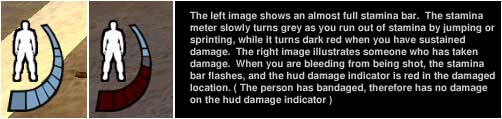
\includegraphics[scale=0.6]{Images/Hud_staminabar.jpg}
    \caption{\small Stamina bar in the HUD of Urban Terror (Source: \cite{urt}).}
    \label{fig:stamina}
  \end{figure}
  
  Two basic techniques will make your movements in the map more efficient: 
  \begin{enumerate}
  \item \emph{Wall jump}: while in the air after a jump or a fall, you can
    bounce on a wall (not necessary in front of you) by pressing jump (default:
    \texttt{SPACE}) when in contact with the wall. 
    You can even repeat this procedure up to 3 times to achieve more complex
    jump and reaching higher places.
  \item \emph{Strafe jump}: this name refers to a common technique in Quake III
    to reach a higher speed. It consists of changing side after each jump during
    a movement\footnote{Note that in Urban Terror and contrary to Quake III, you
      can't keep this procedure for long in a single run because of the stamina
      level.}.   
    For example:
    \begin{itemize}
    \item first sprint or run in a straight or curved line
    \item then jump and and keep turning left + hold left strafe
    \item jump and turn right + right strafe
    \item jump and turn left + left strafe etc. 
    \end{itemize}
    You will probably want to end this sequence by crouching (default key:
    \texttt{C}): it will make your character sliding to maintain the speed for a
    short while. You are able to affect the direction of the sliding using the
    directional key. Another important aspect is that while crouching in this
    way, you don't consume any more stamina and you're able to focus on a given
    point of interest.   
  \end{enumerate}
  For more details and techniques, please refer to the Jumping Guide available
  at \url{http://www.www0.org/cgi-bin/urtj}. 

\item[Exploit H.E. grenades tempo.] 
  Once unlocked, an HE grenade takes around 4 to 5 seconds to explode. You can
  play on this time to decide the best moment to throw it away:
  \begin{itemize}
  \item either immediately to protect a path or a place against incoming
    enemies: hopefully, the grenade will explode while they are reaching the
    place or prevent them from using it for a short while (Note that this also
    applied to HK69);  
  \item or after 3 to 4 seconds such that it explodes when reaching the floor
    such than the ennemy (typically hiden in a corner) won't have time to react
    and move to a safer place.   
  \end{itemize}
  Note that it is possible to unlock a grenade and switch to another weapon to
  cancel the unlocking for further use. This might be useful to avoid team kill
  and a more effective use of them even if I personally consider this as a bug.    
\item[Exploit smoke grenades.] They can cover your movements and be particularly
  effective when used in combination with tactical goggles: you will be able to
  locate incoming enemies and shoot with first strike.    
\end{description}


%----------------------------------
\subsection{Advanced configuration}
\label{sec:client:config}

Apart from the basic key bindings you can operate from the menu \texttt{SETUP}
$\rightarrow$ \texttt{CONTROLS} inside the game, the most useful aspect of UrT
is the capacity to fully customize the commands and the bindings use throughout
the game to reflect your own style of playing.  This is for instance very useful
for the radio commands.  

All the configuration resided in the configuration file \texttt{q3config.cfg},
located in the \texttt{q3ut4/} directory of your installed game, typically:
\begin{itemize}
\item[\windows]  \verb!C:\Program Files\UrbanTerror\q3ut4\!
\item[\linux]    \verb!~/.q3a/q3ut4/! (make sure to show hidden
  directories to find it)
\item [\macosx]  \verb!~/Library/Application Support/Quake3/q3ut4/!
\end{itemize}

\noindent My own configuration file is available at the following url:
\begin{center}
  \url{http://varrette.gforge.uni.lu/q3ut4/q3config.cfg}
\end{center}

\noindent The syntax of this file is inherited from Quake III Arena. I
will only insist on the \emph{binding} procedure. The general use of this
command is: 
\[ bind\  [key]\ "[command]" \]
You may configure multiple commands with a single key: just separate each
commands with a semicolon (;) so that UrT recognizes where each command starts
and stops. 
Note that you can color the text printed in the console using the escape
sequence \verb!^n! where \texttt{n} is a number between 1 and 8 according to the
following associations: 
\begin{center}
  \begin{tabular}[h]{clcl}
    1 & Red    & 2 & Green \\
    3 & Yellow & 4 & Blue  \\
    5 & Purple & 6 & Cyan  \\
    7 & White (Default) & 8 & Black 
  \end{tabular}
\end{center}
Example: "\verb!This text is ^1RED^7 and this one ^8BLACK!"

I will detail in this document the binding of 2 basic commands:
\texttt{ut\_radio} (\S\ref{sub:radio}) and \texttt{ut\_weaptoggle}
(\S\ref{sub:weapons}).  

%.....................................
\subsubsection{Radio command binding}
\label{sub:radio}


The \texttt{ut\_radio} command corresponds to
radio messages (use \texttt{U} to access the radio interface during the game -
see Figure~\ref{fig:radio}) yet it is important to bind the most useful radio
messages on a single key, especially if you want to display a colored message in
the console which is particularly pertinent for bomb site. 
Indeed, while the radio messages refer to them as A and B, they
correspond in practice to bomb site red and black so a colored message will help
your partner to identify more clearly the location you're speaking about.  
      
\begin{figure}[ht]
  \centering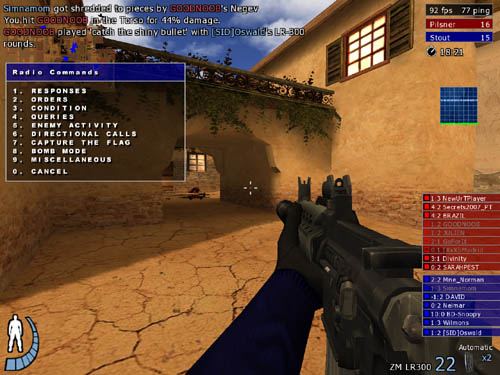
\includegraphics[scale=0.4]{Images/Ui_radiointerface.jpg}
  \caption{\small Radio interface during the game (first level) (Source: \cite{urt}).}
  \label{fig:radio}
\end{figure}

The table~\ref{tab:radio} summarizes the most important messages that justify
(for me) a binding and (eventually), a more pertinent message displayed on the
console. Several variables can be used in such messages, of greater importance stands: 
\begin{itemize}\setitemsep
\item \texttt{\$location}:  current position in the map;
\item \texttt{\$crosshair}: position in the map pointed by your crosshair;
\item \texttt{\$health}:    current health status.
\end{itemize}

Those preliminary comments being done, here is how to use the
table~\ref{tab:radio}. 
For each message, select a key to bind (let's say for instance \texttt{h} to the
radio message asking for a medic) then put the following line in your
\texttt{q3config.cfg}:
\begin{lstlisting}[style=filecontent]
bind h "ut_radio 3 3 I need a medic [^1status: $health^7] @ $location"
\end{lstlisting}
Eventually, if you don't want to overwrite the default message, simply use:
\begin{lstlisting}[style=filecontent]
bind h "ut_radio 3 3"
\end{lstlisting}


%\newcommand{\radio}[1]{\texttt{ut\_radio #1}}
\newcommand{\radio}[1]{\texttt{#1}}

\begin{table}[ht]
  \centering\small
  \begin{tabular}[h]{|c||c|l|}
    \hline
    \textbf{Type} & 
    \textbf{Menu} & \textbf{Proposed Message} \\ 
    \hline\hline
    \multirow{2}{*}{\textbf{Order}} 
                      & \radio{2 5} & \verb!Cover me @ $location! \\ 
                      & \radio{2 6} & \verb!Requesting backup @ $location!\\\hline
    \multirow{4}{*}{\textbf{Questions}}  
                       & \radio{3 2}  & \verb!Awaiting orders! \\ 
                       & \radio{3 3}  & \verb!I need a medic [^1status: $health^7] @ $location!\\
                       & \radio{4 2}  & \verb!Objective status?! \\
                       & \radio{4 4}  & \verb!Where's the enemy?! \\\hline
     \multirow{4}{*}{\textbf{Response}} 
                       & \radio{1 1} & \verb!Affirmative! \\ 
                       & \radio{1 2} & \verb!Negative! \\
                       & \radio{9 4} & \verb!Sorry about that! \\
                       & \radio{9 9} & \verb!Thanks! \\\hline
    \textbf{Activity}     & \radio{5 1} & \verb!Enemy spotted!\\\hline
    \multirow{6}{*}{\textbf{Bomb mode}}
                       & \radio{8 1} & \verb!Heading to bombsite ^1RED!\\
                       & \radio{8 2} & \verb!Heading to bombsite ^8BLACK!\\
                       & \radio{8 3} & \verb!Enemy at bombsite ^1RED!\\
                       & \radio{8 4} & \verb!Enemy at bombsite ^8BLACK!\\
                       & \radio{8 5} & \verb!I have the bomb @ $location!\\
                       & \radio{8 6} & \verb!The bomb is loose!!\\\hline
 
  \end{tabular}
  \caption{Most useful radio message in Urban Terror}
  \label{tab:radio}
\end{table}

You can find the full list of the radio messages in the manual of
UrT~\cite{urt}. 

%.....................................
\subsubsection{Weapon switch binding}
\label{sub:weapon}

By default, the keys 1 to 6 are assigned for the weapons from the knives to the
bomb. It appeared difficult for me to switch quickly with such a configuration
to the sidearm or the knife. That's where the \texttt{ur\_weaptoggle} command is
your friend. 
The format of this command is the following (replace \texttt{x} with the key to assign) : 
\begin{verbatim}
bind x "ut_weaptoggle [argument]"
bind x "ut_weaptoggle [argument] [argument]"
\end{verbatim}
where \texttt{argument} can be one of the following: \texttt{primary},
\texttt{secondary}, \texttt{sidearm}, \texttt{grenade}, \texttt{bomb} or
\texttt{knife}. 

The two argument version permits with the same key to switch from one class of
weapon to another.
For instance, I personally use the following configuration to easily switch from
the primary weapon to the sidearm (useful when in a battle where the magazine
becomes empty) or the knife (for a corporal combat): 
\begin{lstlisting}[style=filecontent]
bind f "ut_weaptoggle sidearm primary"
bind q "ut_weaptoggle knife primary"
\end{lstlisting}

%.......................................................
\subsubsection{Additional sources to tweak your configuration}

I just gave some basic elements of customization. 
You can go further using the following web site: 
\begin{itemize}\setitemsep
\item \url{http://q3ut3.free.fr/gear/} (UrbanTerror Gear script Generator)
  permits the binding of a single key to cycle between several configurations of
  weapons/equipment which can be useful at the beginning of a new map (for
  instance to quickly move from a sniper mod with SR8 to AK).
\item \url{http://ucguides.savagehelp.com/} provides a guide for Quake III where
  some information can be reuse for Urban Terror.
\end{itemize}

%----------------------
\subsection{New maps}

The best way to install new maps is to auto-download them from the server you
are playing. So normally, you have nothing to do (assuming the server is
configured correctly through the \texttt{sv\_dlURL} directive -- see
\S\ref{sec:server:install}).

Yet, you may want to install manually new maps. 
Apart from the basic maps, you can find community created levels on the
following website (ordered by personal preferences):
\begin{itemize}\setitemsep
\item \url{http://www.snipersgaulois.com/downloads.php}
\item \url{http://sex-e.clanservers.com/Downloads/c=1.html}
\item \url{http://urt.unfoog.de/q3ut4/}
\end{itemize}

Just put them into your \texttt{q3ut4/} directory.

Those sites propose in general a huge number of maps, some buggy and/or
unfinished. If you're only interested in pre-tested maps, you can take a look at
my own repository available at: \url{http://varrette.gforge.uni.lu/q3ut4/}




%~~~~~~~~~~~~~~~~~~~~~~~~~~~~~~~~~~~~~~~~~~~~~~~~~~~~~~~~~~~~~~~~
% eof
%
% Local Variables:
% fill-column: 80
% mode: latex
% mode: flyspell
% mode: auto-fill
% End:
